\documentclass[a4paper,14pt]{article}
\usepackage[warn]{mathtext} %для поддержки кириллицы в формулах
\usepackage{amsmath} %основной пакет для формул
\usepackage[utf8x]{inputenc}
\usepackage[T1,T2A]{fontenc}
\usepackage[russian]{babel}
\usepackage{hyperref}
\usepackage{indentfirst}
\usepackage{listings}
\usepackage{color}
\usepackage{here}
\usepackage{array}
\usepackage{multirow}
\usepackage{graphicx}

\usepackage{caption}
\renewcommand{\lstlistingname}{Программа} % заголовок листингов кода

\usepackage{listings}
\lstset{ %
extendedchars=\true,
keepspaces=true,
language=bash,					% choose the language of the code
basicstyle=\footnotesize,		% the size of the fonts that are used for the code
numbers=left,					% where to put the line-numbers
numberstyle=\footnotesize,		% the size of the fonts that are used for the line-numbers
stepnumber=1,					% the step between two line-numbers. If it is 1 each line will be numbered
numbersep=5pt,					% how far the line-numbers are from the code
backgroundcolor=\color{white},	% choose the background color. You must add \usepackage{color}
showspaces=false				% show spaces adding particular underscores
showstringspaces=false,			% underline spaces within strings
showtabs=false,					% show tabs within strings adding particular underscores
frame=single,           		% adds a frame around the code
tabsize=2,						% sets default tabsize to 2 spaces
captionpos=b,					% sets the caption-position to bottom
breaklines=true,				% sets automatic line breaking
breakatwhitespace=false,		% sets if automatic breaks should only happen at whitespace
escapeinside={\%*}{*)},			% if you want to add a comment within your code
postbreak=\raisebox{0ex}[0ex][0ex]{\ensuremath{\color{red}\hookrightarrow\space}}
}

\usepackage[left=2cm,right=2cm,
top=2cm,bottom=2cm,bindingoffset=0cm]{geometry}


\begin{document}	% начало документа

\begin{titlepage}	% начало титульной страницы

	\begin{center}		% выравнивание по центру

		\large Санкт-Петербургский политехнический университет Петра Великого\\
		\large Институт компьютерных наук и технологий \\
		\large Кафедра компьютерных систем и программных технологий\\[1cm]
		
		\includegraphics[scale=0.7]../pics/spbpu.jpg}\\[2cm]
		
		\huge Реферат по компьютерной алгебре\\[0.5cm] % название работы, затем отступ 0,5см
		\huge Алгоритмы сжатия изображений\\[3cm]

	\end{center}	
	
	\begin{flushright} % выравнивание по правому краю
		\begin{minipage}{0.25\textwidth} % врезка в половину ширины текста
			\begin{flushleft} % выровнять её содержимое по левому краю

				\large\textbf{Студенты:}\\
				\large В.В. ~Дьячков\\
				\large А.А. ~Жуйков\\
				\large А.Ю. ~Ламтев\\
				\large Ю.И. ~Леженин\\
				\large {Группа:} 13501/4\\
				
				\large \textbf{Преподаватель:}\\
				\large И.А. ~Малышев\\

			\end{flushleft}
		\end{minipage}
	\end{flushright}
	
	\vfill % заполнить всё доступное ниже пространство

	\begin{center}
	\large Санкт-Петербург\\
	\large \the\year % вывести дату
	\end{center} % закончить выравнивание по центру
\thispagestyle{empty} % не нумеровать страницу
\end{titlepage} % конец титульной страницы

\vfill % заполнить всё доступное ниже пространство



% Содержание
%\tableofcontents
\newpage


\section*{Введение}

Сейчас мы живем в информационном обществе, и нас окружает огромный объем информации в том числе и графической. Наверно хоть раз вы отправляли картинку своему приятелю в социальной сети. Цифровое изображение при хранении занимает большие объемы памяти. Так растровое изображение размером 1024 на 1024 пикселов с глубиной цвета 24 бит занимает 3 Мб. Понятно, что хранение и передача изображений в таком виде является весьма трудоёмкой задачей. Поэтому задача представления изображений в компактной форме (сжатие данных) является весьма актуальной. При этом должны быть разработаны алгоритмы как для кодирования, так и для декодирования (восстановления) изображений. 
	
Первыми для архивации изображений стали применяться привычные алгоритмы. Те, что использовались и используются в системах резервного копирования, при создании дистрибутивов и т.п. Эти алгоритмы архивировали информацию без изменений. Однако основной тенденцией в последнее время стало использование новых классов изображений. Старые алгоритмы перестали удовлетворять требованиям, предъявляемым к архивации. Многие изображения практически не сжимались, хотя “на взгляд” обладали явной избыточностью. Это привело к созданию нового типа алгоритмов — сжимающих с потерей информации. Как правило, коэффициент архивации и, следовательно, степень потерь качества в них можно задавать. При этом достигается компромисс между размером и качеством изображений.
	
Идея, лежащая в основе всех алгоритмов сжатия с потерями, довольно проста: на первом этапе удалить несущественную информацию, а на втором этапе к оставшимся данным применить наиболее подходящий алгоритм сжатия без потерь. Основные сложности заключаются в выделении этой несущественной информации. Подходы здесь существенно различаются в зависимости от типа сжимаемых данных. Для звука чаще всего удаляют частоты, которые человек просто не способен воспринять, уменьшают частоту дискретизации, а также некоторые алгоритмы удаляют тихие звуки, следующие сразу за громкими, для видеоданных кодируют только движущиеся объекты, а незначительные изменения на неподвижных объектах просто отбрасывают. Методы выделения несущественной информации на изображениях будут подробно рассмотрены далее.

\section*{Методы сжатия}
\subsection*{Квантование и дискретезация}
https://habrahabr.ru/post/251417/
С процессом квантования и дискретизации связано понятие визуальной избыточности. Значительная часть информации на изображении не может быть воспринята человеком: например, человек способен замечать незначительные перепады яркости, но гораздо менее чувствителен к цветности. Также, начиная с определённого момента, повышение точности дискретизации не влияет на визуальное восприятие изображения. Таким образом, некоторая часть информации может быть удалена без ухудшения визуального качества. Такую информацию называют визуально избыточной.
Самым простым способом удаления визуальной избыточности является уменьшение точности дискретизации, но на практике этот способ можно применять только для изображений с простой структурой, т.к. искажения, возникающие на сложных изображениях, слишком заметны см рис \ref{pic:discretization}.

\begin{figure}[H]
	\begin{center}
		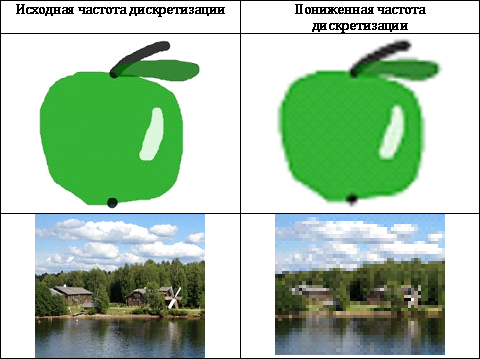
\includegraphics[scale=0.9]{pics/quantization/discretization.png}
		\caption{Уменьшение точности дискретизации} 
		\label{pic:discretization}
	\end{center}
\end{figure}
Для удаления избыточной информации чаще уменьшают точность квантования, но нельзя уменьшать её бездумно, т.к. это приводит к резкому ухудшению качества изображения. Предположим, что изображение представлено в цветовом пространстве RGB, результаты кодирования этого изображения с пониженной точностью квантования представлены на рис \ref{pic:levelsOfQuantization}.
\begin{figure}[H]
	\begin{center}
		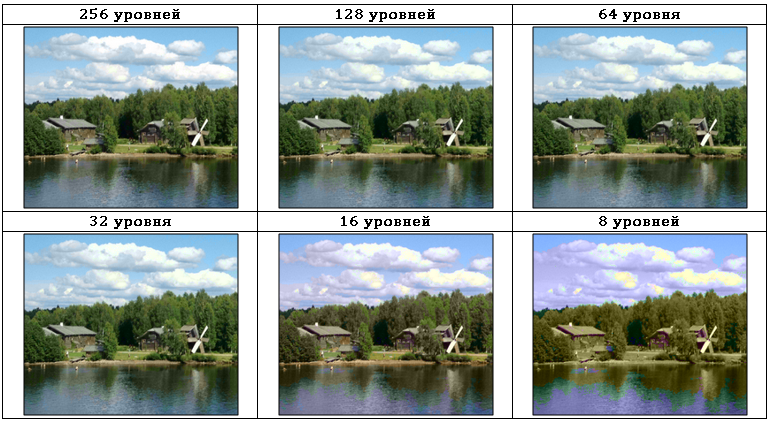
\includegraphics[scale=0.85]{pics/quantization/levelsOfQuantization.png}
		\caption{Уменьшение точности квантования} 
		\label{pic:levelsOfQuantization}
	\end{center}
\end{figure}
Внимательно изучив полученные изображения, можно заметить, что на сжатых изображениях возникают отчётливые ложные контуры, которые значительно ухудшают визуальное восприятие. Существуют методы, основанные на переносе ошибки квантования в следующий пиксел, позволяющие значительно уменьшить или даже совсем удалить эти контуры, но они приводят к зашумлению изображения и появлению зернистости. Перечисленные недостатки сильно ограничивают прямое применение квантования для сжатия изображений.
Большинство современных методов удаления визуально избыточной информации используют сведения об особенностях человеческого зрения. Всем известна различная чувствительность человеческого глаза к информации о цветности и яркости изображения. На рис \ref{pic:quantization} показано изображение в цветовом пространстве YIQ, закодированное с разной глубиной квантования цветоразностных сигналов IQ:
\begin{figure}[H]
	\begin{center}
		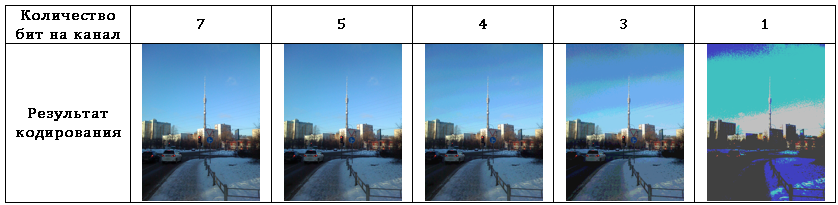
\includegraphics[scale=0.75]{pics/quantization/quantization.png}
		\caption{Различная глубина квантования цветоразностных сигналов IQ} 
		\label{pic:quantization}
	\end{center}
\end{figure}
Как видно из рис \ref{pic:quantization}, глубина квантования цветоразностных сигналов может быть понижена с 256 до 32 уровней с минимальными визуальными изменениями. В то же время потери в I и Q составляющих весьма существенны. Несмотря на простоту описанных методов, в чистом виде они применяются редко, чаще всего они служат одним из шагов более эффективных алгоритмов.

\subsection*{Вейвлет сжатие}
%source: https://habrahabr.ru/post/251417/
Вейвлеты – математические функции, предназначенные для анализа частотных компонент данных. В задачах сжатия информации вейвлеты используются сравнительно недавно, тем не менее исследователям удалось достичь впечатляющих результатов.
В отличие от рассмотренных выше преобразований, вейвлеты не требуют предварительного разбиения исходного изображения на блоки, а могут применяться к изображению в целом. В данном разделе вейвлет сжатие будет пояснено на примере довольно простого вейвлета Хаара.
Для начала рассмотрим преобразование Хаара для одномерного сигнала. Пусть есть набор S из n значений, при преобразовании Хаара каждой паре элементов ставится в соответствие два числа: полусумма элементов и их полуразность. Важно отметить, что это преобразование обратимо: т.е. из пары чисел можно легко восстановить исходную пару. На рис \ref{pic:wavelet_example} показан пример одномерного преобразования Хаара:
\begin{figure}[H]
	\begin{center}
		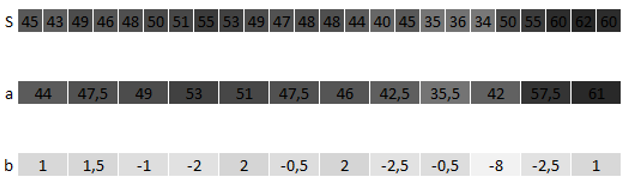
\includegraphics[scale=0.9]{pics/wavelet/example.png}
		\caption{Пример для одномерного пространства} 
		\label{pic:wavelet_example}
	\end{center}
\end{figure}
Видно, что сигнал распадается на две составляющее: приближенное значение исходного (с уменьшенным в два раза разрешением) и уточняющую информацию.
Двумерное преобразование Хаара – простая композиция одномерных преобразований. Если исходные данные представлены в виде матрицы, то сначала выполняется преобразование для каждой строки, а затем для полученных матриц выполняется преобразование для каждого столбца. На рис \ref{pic:wavelet_compression} показан пример двумерного преобразования Хаара.

\begin{figure}[H]
	\begin{center}
		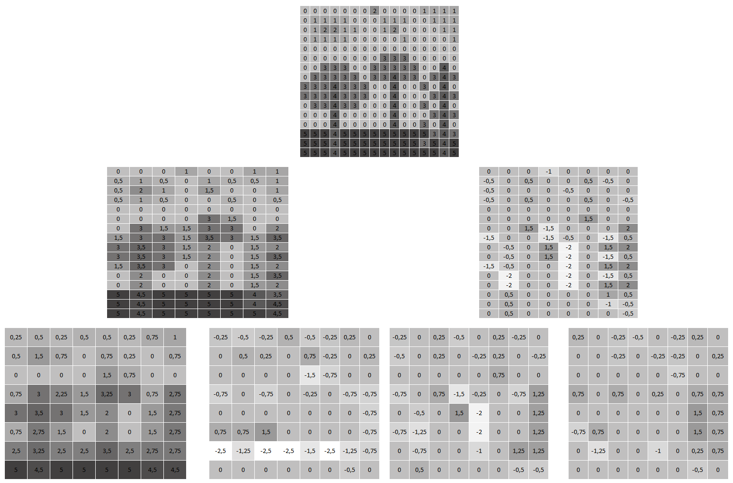
\includegraphics[scale=0.7]{pics/wavelet/compression.png}
		\caption{Процесс сжатия} 
		\label{pic:wavelet_compression}
	\end{center}
\end{figure}
Цвет пропорционален значению функции в точке (чем больше значение, тем темнее). В результате преобразования получается четыре матрицы: одна содержит аппроксимацию исходного изображения (с уменьшенной частотой дискретизации), а три остальных содержат уточняющую информацию.
Сжатие достигается путём удаления некоторых коэффициентов из уточняющих матриц. На рис \ref {pic:wavelet_uncompression} показан процесс восстановления и само восстановленное изображение после удаления из уточняющих матриц малых по модулю коэффициентов:

\begin{figure}[H]
	\begin{center}
		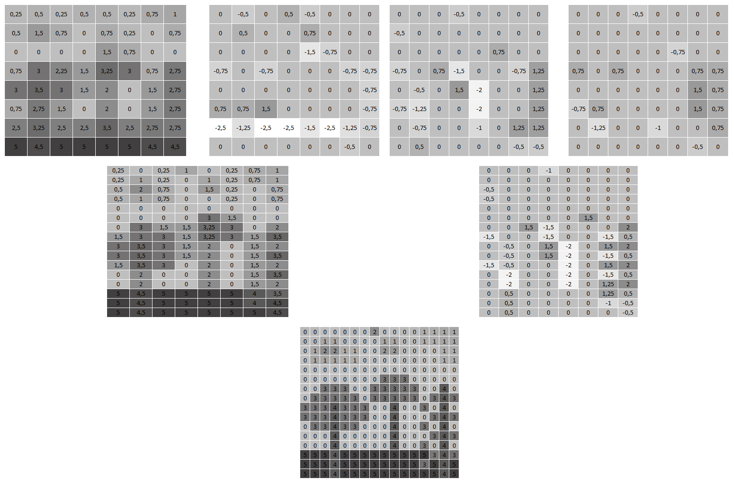
\includegraphics[scale=0.7]{pics/wavelet/uncompression.png}
		\caption{Процесс восстановления} 
		\label{pic:wavelet_uncompression}
	\end{center}
\end{figure}
Очевидно, что представление изображения с помощью вейвлетов позволяет добиваться эффективного сжатия, сохраняя при этом визуальное качество изображения. Существуют и другие вейвлеты, с помощью которых производится сжатие изображений.

\subsection*{RLE}
%source: https://habrahabr.ru/post/251417/
Все алгоритмы серии RLE основаны на очень простой идее: повторяющиеся группы элементов заменяются на пару (количество повторов, повторяющийся элемент). Рассмотрим этот алгоритм на примере последовательности бит. В этой последовательности будут чередовать группы нулей и единиц. Причём в группах зачастую будет более одного элемента. Тогда последовательности 11111 000000 11111111 00 будет соответствовать следующий набор чисел 5 6 8 2. Эти числа обозначают количество повторений (отсчёт начинается с единиц), но эти числа тоже необходимо кодировать. Будем считать, что число повторений лежит в пределах от 0 до 7 (т.е. нам хватит 3 бит для кодирования числа повторов). Тогда рассмотренная выше последовательность кодируется следующей последовательностью чисел 5 6 7 0 1 2. Легко подсчитать, что для кодирования исходной последовательности требуется 21 бит, а в сжатом по методу RLE виде эта последовательность занимает 18 бит.
Хоть этот алгоритм и очень прост, но эффективность его сравнительно низка. Более того, в некоторых случаях применение этого алгоритма приводит не к уменьшению, а к увеличению длины последовательности. Для примера рассмотрим следующую последовательность 111 0000 11111111 00. Соответствующая ей RL-последовательность выглядит так: 3 4 7 0 1 2. Длина исходной последовательности – 17 бит, длина сжатой последовательности – 18 бит.
Этот алгоритм наиболее эффективен для чёрно-белых изображений. Также он часто используется, как один из промежуточных этапов сжатия более сложных алгоритмов.
\section*{Картинка}

\begin{figure}[H]
	\begin{center}
		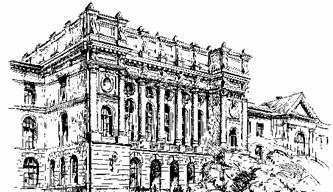
\includegraphics[scale=0.7]{pics/spbpu.jpg}
		\caption{название картинки} 
		\label{pic:pic_name} % название для ссылок внутри кода
	\end{center}
\end{figure}

\section*{Выводы}
Всё круто!!!

\end{document}
